Ein Federkatapult stösst einen Klotz von \mKO\ auf einem waagrechten, reibungsfreien Boden weg. Die Feder (Federkonstante \kKO) ist anfangs um \sKO\ zusammengedrückt. Zustand (1): Feder zusammengedrückt, Klotz in Ruhe; (2): Feder nur noch um die Hälfte, $s/2$, zusammengedrückt; (3): Feder entspannt, der Klotz hat sie verlassen und gleitet weiter.
\begin{center}
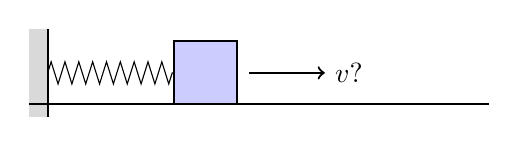
\begin{tikzpicture}[scale=0.8]
 \fill[gray!30] (-0.3,-0.2) rectangle (0,1.2);
 \draw[thick] (0,-0.2) -- (0,1.2);
 \draw[thick] (-0.3,0) -- (7,0);
 \draw[decorate, decoration={zigzag, segment length=5, amplitude=4}] (0,0.5) -- (2,0.5);
 \draw[thick, fill=blue!20] (2,0) rectangle (3,1);
 \draw[->, thick] (3.2,0.5) -- (4.4,0.5) node[right] {$v$?};
\end{tikzpicture}
\end{center}
Ein Schüler füllt diese Energietabelle aus:
\begin{center}
\begin{tabular}{lcc}
 & $E_\mathrm{el}$ & $E_\mathrm{kin}$ \\ \hline
 (1) Feder zusammengedrückt & \EaP{0}{3} & \SI{0}{\joule} \\
 (2) Feder um $s/2$ zusammengedrückt & \EebP{0}{3} & \EkbP{0}{3} \\
 (3) Klotz hat die Feder verlassen & \EaP{0}{3} & \EaP{0}{3}
\end{tabular}
\end{center}

\begin{abcliste}
\abc
Ein Eintrag der Tabelle ist falsch. Welcher? Was wäre richtig?

\abc
Prüfe die Zeile (2): Warum ist die Spannenergie dort nur ein Viertel der Anfangsenergie und nicht die Hälfte?

\abc
Wie schnell ist der Klotz in (2) und in (3)?

\abc
Eine Mitschülerin rechnet in (1) $E_\mathrm{el} = \frac{1}{2}\,k\,s = \frac{1}{2}\cdot\kK\cdot\sK \approx \SI{12.3}{\joule}$. Woran erkennt man sofort, dass das nicht stimmt?
\end{abcliste}
